%!TeX root=../tese.tex
%("dica" para o editor de texto: este arquivo é parte de um documento maior)
% para saber mais: https://tex.stackexchange.com/q/78101

% Vamos definir alguns comandos auxiliares para facilitar.

% "textbackslash" é muito comprido.
\newcommand{\sla}{\textbackslash}

% Vamos escrever comandos (como "make" ou "itemize") com formatação especial.
\newcommand{\cmd}[1]{\textsf{#1}}

% Idem para packages; aqui estamos usando a mesma formatação de \cmd,
% mas poderíamos escolher outra.
\newcommand{\pkg}[1]{\textsf{#1}}

% A maioria dos comandos LaTeX começa com "\"; vamos criar um
% comando que já coloca essa barra e formata com "\cmd".
\newcommand{\ltxcmd}[1]{\cmd{\sla{}#1}}

\chapter{Data Ingestion Study Case}
\label{chap:dataingestion}

\section{Introduction}
\label{sec:introduction}
OpenDataHub (ODH) is a digital platform that makes data from different sources available in a standardized pattern, removing the complexity from integrating multiple data sources for the users. The full picture of their system can be split on three functionalities:

\begin{itemize}
    \item Data ingestion: applications responsible for retrieving or receiving data from external data sources, identifying, transforming and storing it.
    \item Data storage: the data is stored in as stations and values, where stations can contain other stations or values, and values are measurements ingested. For example, a charging plug station is a station that contains plugs, each plug is a station that contains a value ”available” or “not available”. Stations can contain more than one value, for example, a latitude-longitude point is a station that contain values for wind speed, wind direction, air pressure, and others. These values are stored in the same unit for every station, no matter the original data source unit and format.
    \item Data exposure: a common API to make data from stations available for end users.
\end{itemize}

This case study focuses on the data ingestion architecture, and how to increase its extensibility.

\begin{figure}
    \centering
    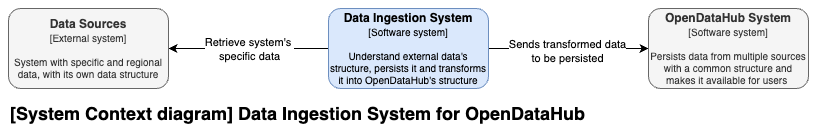
\includegraphics[width=1\textwidth]{collector-consumer-CONTEXT.drawio}
    \caption{Data Ingestion context diagram.\label{fig:subfigures}}
\end{figure}

\section{Current architecture}
\label{sec:current}

The ODH's data collectors architecture initial requirement is to connect to different data sources, using different protocols (e.g. HTTP APIs, MQTT, FTP) to download the data, aggregate and transform it to the stations-value pattern, and save it on ODH’s storage.

The current architecture uses independent applications dedicated to each data source. Each application is responsible for connecting to the data source, retrieving the data, aggregating and/or transforming it, and sending it to ODH's system for persisting data.

\begin{figure}
    \centering
    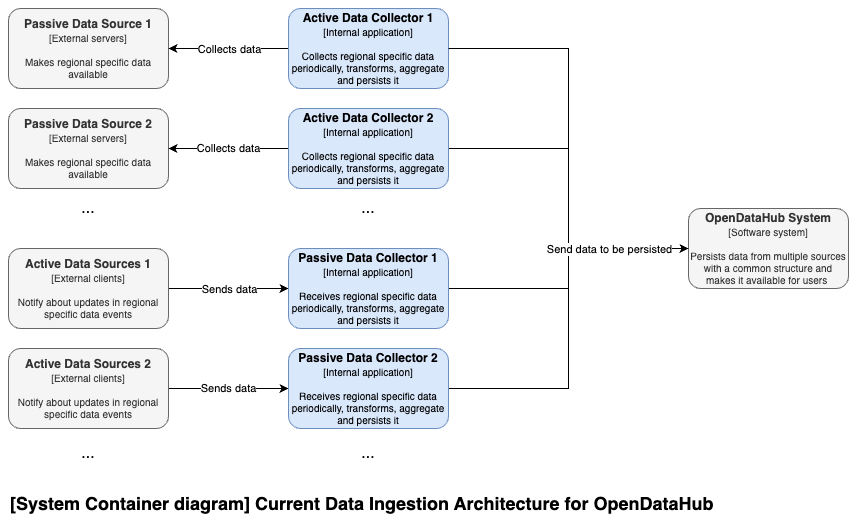
\includegraphics[width=1\textwidth]{collector-consumer-OLD CONTAINERS.drawio}
    \caption{Data Ingestion current architecture containers diagram.\label{fig:subfigures}}
\end{figure}

This solution contains a problem of redundant work for each data collector service: they all have code to connect with the ODH's persistence system and might benefit from reusing processing and transformation tooling. This creates N dependencies with the storage, consequently, if there is a change in how the connection with the ODH's persistence system is made, it would require changing every data collector.

Besides, to integrate a new data source to the data collection, it is necessary to create a new service with collecting, parsing, transforming, and persisting code.

\section{New requirements}
\label{sec:requirements}

As a growing platform, ODH wants to be able to integrate new data sources with ease, decreasing technical requirements and development time. As part of this, it is essential to provide a way for data sources' teams to integrate with ODH's data collection, without requiring (or at least reducing) ODH's technical team involvement.

Furthermore, it is essential to have a way to track and debug the ingestion flow. For this reason, another requirement is to integrate a new database to store the “raw” data, which means, the data as it is collected, before it is transformed into the ODH stations pattern.

For this, the current architecture would require each data collector application to connect to the raw data storage and store it. Creating another dependency coupling problem, since every data collector would require a dependency with the Raw data storage.

\section{Proposed architecture}
\label{sec:proposed}

The new architecture proposed in this thesis aims to increase the system extensibility by reducing development time to create new data collectors. With it, it creates an option for data sources that want to integrate in, reducing ODH's technical team involvement and removing data collectors coupling with storage systems.

The new architecture uses microservices and asynchronous communication to modularize and split concerns along the system. (Figure~\ref{fig:containers})

\begin{figure}
    \centering
    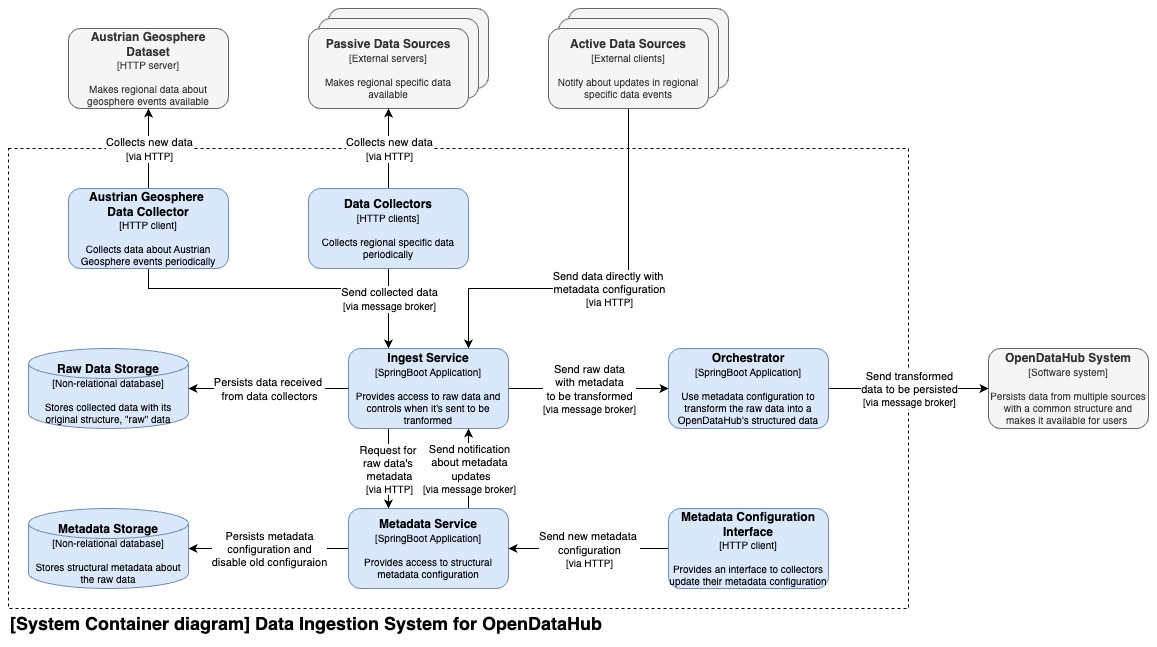
\includegraphics[width=1\textwidth]{collector-consumer-CONTAINERS.drawio}
    \caption{Data Ingestion proposed architecture containers diagram.\label{fig:containers}}
\end{figure}

The biggest challenge in this architecture is: How to treat external data and their singularities? Each data source have its own data format and structure, how to extract the information needed by ODH and transform it into the expected pattern?

It can be solved with structural metadata, metadata is a kind of data used to describe data, in this case it will contain information about the data structure: in which field is an important value, what is are the data types and how to access each wanted value.

This metadata can be sent with the data or configured, in case the same metadata can be used multiple times and is needed for the transformation process.

\subsection{Ingestion}
\label{sec:ingestion}

The data ingestion is done by the Ingestion Service. It is responsible for receiving the raw data from data collectors or active data sources (data sources sending the data directly to it), persisting this data into a raw data storage, and sending data to be transformed.

Data can only be sent to be processed once there is a metadata configuration to it. This metadata can be sent with the data, or be fetched from the Metadata Service (application responsible for handling metadata operations).

However, the raw data persistence does not depend on the metadata configuration. This means that, a data received without metadata and that doesn't have any metadata configuration, will be persisted on Raw Data Storage and send for transformation once the metadata is configured. For this reason, there is a dedicated worker to listen for metadata update messages and trigger this process. (Figure~\ref{fig:ingest})

\begin{figure}
    \centering
    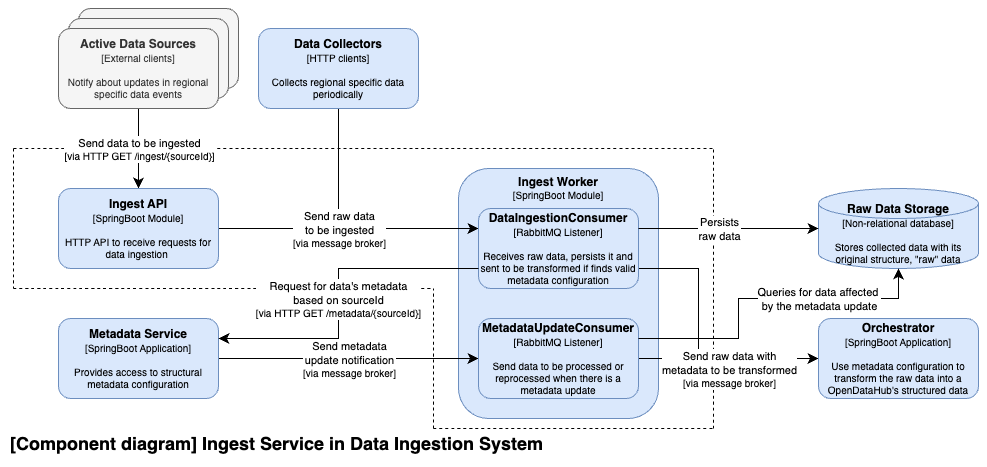
\includegraphics[width=1\textwidth]{collector-consumer-COMPONENT INGEST.drawio}
    \caption{Ingestion service components diagram.\label{fig:ingest}}
\end{figure}

\subsection{Metadata}
\label{sec:ingestion}

The solution uses structural metadata about the data ingested to transform data from its raw structure into the ODH's stations pattern. This metadata can be sent or collected with the data, or can be configured to be applied on data collected during a time range.

There is a metadata storage to store active configurations and to help debugging. The application dedicated to handle access and operations on the storage is the Metadata Service.

There is also a Metadata Configuration Interface to help developers and data sources to configure new metadata and manage their data configuration. (Figure~\ref{fig:metadata})

\begin{figure}
    \centering
    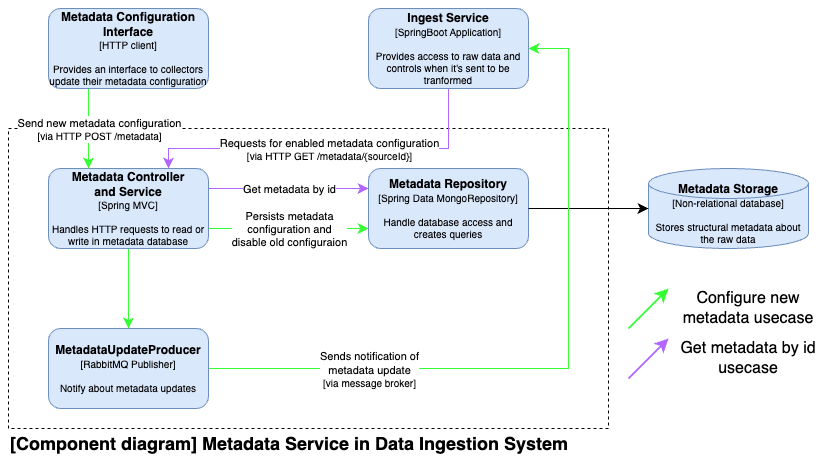
\includegraphics[width=1\textwidth]{collector-consumer-COMPONENT METADATA.drawio}
    \caption{Metadata service components diagram.\label{fig:metadata}}
\end{figure}

The metadata is built with a common structure and stored as a json. Follows a example of metadata in Program~\ref{prog:metadata}.

\begin{program}
    \index{JSON}
    \centering
  
  \begin{lstlisting}[language=JSON, style=wider]
{
  "sourceId": "austrian-geosphere",
  "startDate": "2015-08-04T10:11:30",
  "expirationDate": "2029-08-04T10:11:30",
  "metadata": {
    "dataId": "austrian-geosphere-data",
    "origin": "austrian-geosphere-data-collector",
    "period": 600,
    "timestampProperty": "timestamps.0",
    "results": {
      "type": "array",
      "property": "features",
      "idProperty": "properties.station"
    },
    "stations": {
      "type": "array",
      "property": "features",
      "identification": {
        "property": "properties.station"
      },
      "location": {
        "property": "geometry.coordinates",
        "type": "array",
        "longitude": "0",
        "latitude": "1"
      }
    },
    "datatypes": [
      {
        "datatypeName": "air_pressure",
        "method": "extract",
        "unitProperty": "properties.parameters.P.unit",
        "valueProperty": "properties.parameters.P.data",
        "targetUnit": "hPa",
        "rtype": "mean"
      },
      {
        "datatypeName": "wind_speed",
        "method": "extract",
        "unitProperty": "properties.parameters.FF.unit",
        "valueProperty": "properties.parameters.FF.data",
        "targetUnit": "m/s",
        "rtype": "mean"
      },
      {
        "datatypeName": "wind_direction",
        "method": "extract",
        "unitProperty": "properties.parameters.DD.unit",
        "valueProperty": "properties.parameters.DD.data",
        "targetUnit": "°",
        "rtype": "mean"
      },
      {
        "datatypeName": "wind_temperature",
        "method": "extract",
        "unitProperty": "properties.parameters.TL.unit",
        "valueProperty": "properties.parameters.TL.data",
        "targetUnit": "°F",
        "rtype": "mean"
      }
    ]
  }
}
  \end{lstlisting}
  
    \caption{Structural metadata for Austrian Geosphere dataset.\label{prog:metadata}}
\end{program}

The content describes how the data structure and in which keys are key values for the data transformation, for example: the timestamp of the event, the event location and the value registered.

\subsection{Transformation}
\label{sec:transformation}

The data transformation is done by the Orchestrator, once it receives data with its metadata configuration. The Orchestrator uses the metadata to understand the particularities of the raw data and transform it into the ODH's stations structure.

The Orchestrator is not only responsible for transforming the data structure to match the expected structure, but also to transform the collected value into the expected unit of measurement. Since, the data is stored in the same unit to ease end users. It can do so, by using the Transformers.

Transformers are small pieces of code that do only one transformation into the value. For example, there may be a Transformer to transform a temperature value measured in Celsius to Kelvin. The Orchestrator is responsible for selecting the correct Transformers and running them into the correct order to transform from the collected unit to the one used by ODH's system. (Figure~\ref{fig:orchestrator})

\begin{figure}
    \centering
    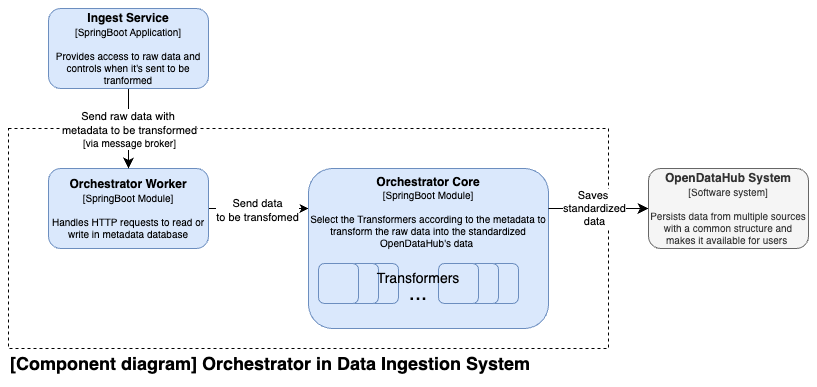
\includegraphics[width=1\textwidth]{collector-consumer-COMPONENT ORCHESTRATOR.drawio}
    \caption{Orchestrator components diagram.\label{fig:orchestrator}}
\end{figure}

\section{Experiment}
\label{sec:exp}

There is an experiment to test the proposed architecture. It simulates the integration of an Austrian geosphere data source, it ingests data of currently air pressure, temperature, wind speed and direction in difference points from Austria. The data is collected every 10 minutes, the time the data source takes to update its values. This experiment aims to only simulate the data ingestion process and do not send data to be persisted in the ODH system, but it allows observing the products of data ingestion and how each microservice relates and communicates with each other.

The experiment is in a GitHub repository as a Gradle monorepo, each service is a submodule of the repository, but each one can be deployed individually as a microservice, they are in Java 17. They use SpringBoot to create HTTP APIs and asynchronous workers. For infrastructure, it uses MongoDB for data storage and RabbitMQ for asynchronous communication via message queues.

To run the experiment, it is necessary to first prepare the environment, then run the infrastructure; after that, run the microservices, and finally include test metadata. It is also possible to simulate an active data source and send data directly to it to be ingested. This process is described step-by-step on the repository's README.

To access the HTTP endpoints, it is possible to use the Postman collection available in the repository, to act as an interface for debugging, active data ingestion and/or metadata configuration.

During the experiment run, the applications logs are directed to files in the log folder to ease debugging and tracking. It is also possible to access the MongoDB, to track the data stored, and the RabbitMQ, to track messages and queues, servers by using the values into the docker-compose file.

\section{Takeaways}
\label{sec:conc}

It is possible to evaluate extensibility on a data ingestion system by how easy it is to integrate different data sources and give maintenance to it.

On the current architecture, integrating a different data source would require creating a new application that would collect the data, transform and send it to ODH. Every time the data changes, it would require change on the code base, this requires effort from the ODH's technical team and alignment with between ODH and the data source owners.

The proposed architecture uses microservices and the concept of modularity to split the responsibility between the system in different microservices. Also uses structural metadata to abstract transformation logic from the data collector.

For these reasons, to integrate a new data source on the proposed architecture requires less technical work, once it is possible to be integrated by the own data source, via the ingestion API, or requires a data collector service that only contains code related to data collecting.

Also, maintaining the data sources is much easier, since data changes can be instantly met in the transformation process by changing the metadata configuration, that can be done by the own data source team, via the metadata service API, reducing ODH technical team involvement.

Another advantaged brought by the proposed architecture is the use of asynchronous communication. This reduces coupling problems, once the message publisher doesn't have any dependency with the consumer application. It also increases scalability, by reducing the harm of overload scenarios, since the messages are stored and only processed by the consumer once it is available.

A further improvement of the proposed architecture is the split of ingestion and transformation flows. Ingestion is the process of collecting the data and persisting it in the Raw Data Storage, and the transformation is the process of using metadata to transform raw data into ODH's standardized data. Separating them, means that data can be ingested even thought they are not ready to be transformed (doesn't have a metadata configuration). This increases the data collecting capability, since it is not attached to the transformation logic, and reduce risks of data loss, once the data is stored and is going to be processed once the metadata is configured.

This also prevent for unexpected behaviors on transformation to cause data loss, because the raw data is stored, and once the cause is found and fixed, the transformation can be triggered again.

Although there are many advantages with the proposed architecture, the use of asynchronous communication, microservices and the addition of two data storage cause an increase in infrastructure cost and maintainability. For this reason, it is important to be sure there is an experienced team with microservices and the use of observability and tracking tools, such as Grafana, Prometheus and Sentry, to make sure that the applications are healthy and working as intended and any unwanted behavior is caught and fixed as soon as possible.
